%
% problemstellung.tex -- Beispiel-File für die Beschreibung des Problems
%
% (c) 2020 Prof Dr Andreas Müller, Hochschule Rapperswil
%
\section{Problemstellung
\label{steps:section:problemstellung}}
\rhead{Problemstellung}
Die Schrittweitensteuerung soll dazu dienen, numerische Berechnungen von Differenzialgleichungen (z.B. Runge-Kutta Verfahren) zu beschleunigen.
Um die optimale Schrittlänge zu bestimmen ist eine Fehlerschätzung nötig,
was jedoch auch Rechenleistung beansprucht.
Aus diesem Dilemma stammt auch einer der wichtigsten Knackpunkte des Themas:
Wie findet man die optimale Schrittlänge, ohne zuviel Rechenpower dafür zu verschwenden?
Denn wenn zuviel Energie in das Finden der optimalen Schrittweite gesteckt wird,
ist der Gewinn im Vergleich zu einer fixen, kleineren Schrittlänge zunichte.
\begin{equation}
\int_a^b x^2\, dx
=
\left[ \frac13 x^3 \right]_a^b
=
\frac{b^3-a^3}3.
\label{steps:equation1}
\end{equation}
\begin{figure}
\centering
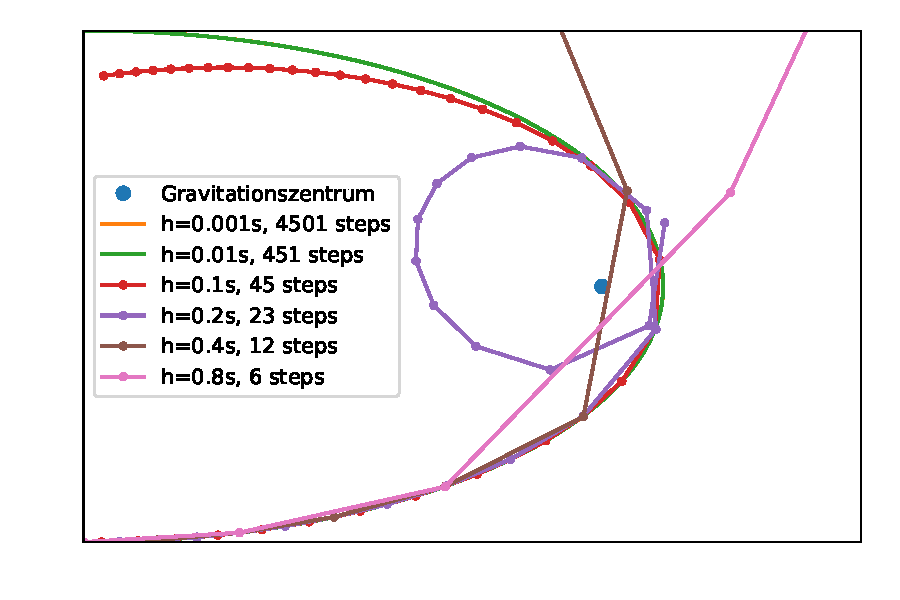
\includegraphics{papers/steps/img/gravity_different_fixed_stepsize.pdf}
\caption{Bahn eines Teilchens, von unten rechts kommend,
um ein Gravitationszentrum, berechnet mit unterschiedlichen Schrittweiten.
Zweidimensionale DGL zweiter Ordnung:
$a(t)=P''(t)=\frac{Pfix-P(t)\cdot m\cdot g}{|Pfix-P(t)|^{3}}$
mit $P(0)=(0, 0)$, $Pfix(2, 1)$, $P'(0)=v(0)=(0.669, 0)$, $g=1$, $m=1$
\label{buch:steps:fixed_comparison}}
\end{figure}
Die hier behandelten Beispiele basieren alle auf einem Runge-Kutta Verfahren
vierter Ordnung. Zur veranschaulichung, welche Wirkung verschiedene Schrittgrössen
auf das Resultat haben können, wird in Grafik~\ref{buch:steps:fixed_comparison} aufgezeigt.


%\subsection{De finibus bonorum et malorum
%\label{steps:subsection:finibus}}
%\ref{steps:section:folgerung}.



